\section*{Teoretická část}

K pokusu používáme aparaturu znázorněnou na obrázku \ref{obr:zfp-nakres}. Vodorovná trubice má vnitřní poloměr $r$ a ve vzdálenosti $l$ od ústí je umístěna manometrická trubice.

\begin{figure}[h] 
\centering
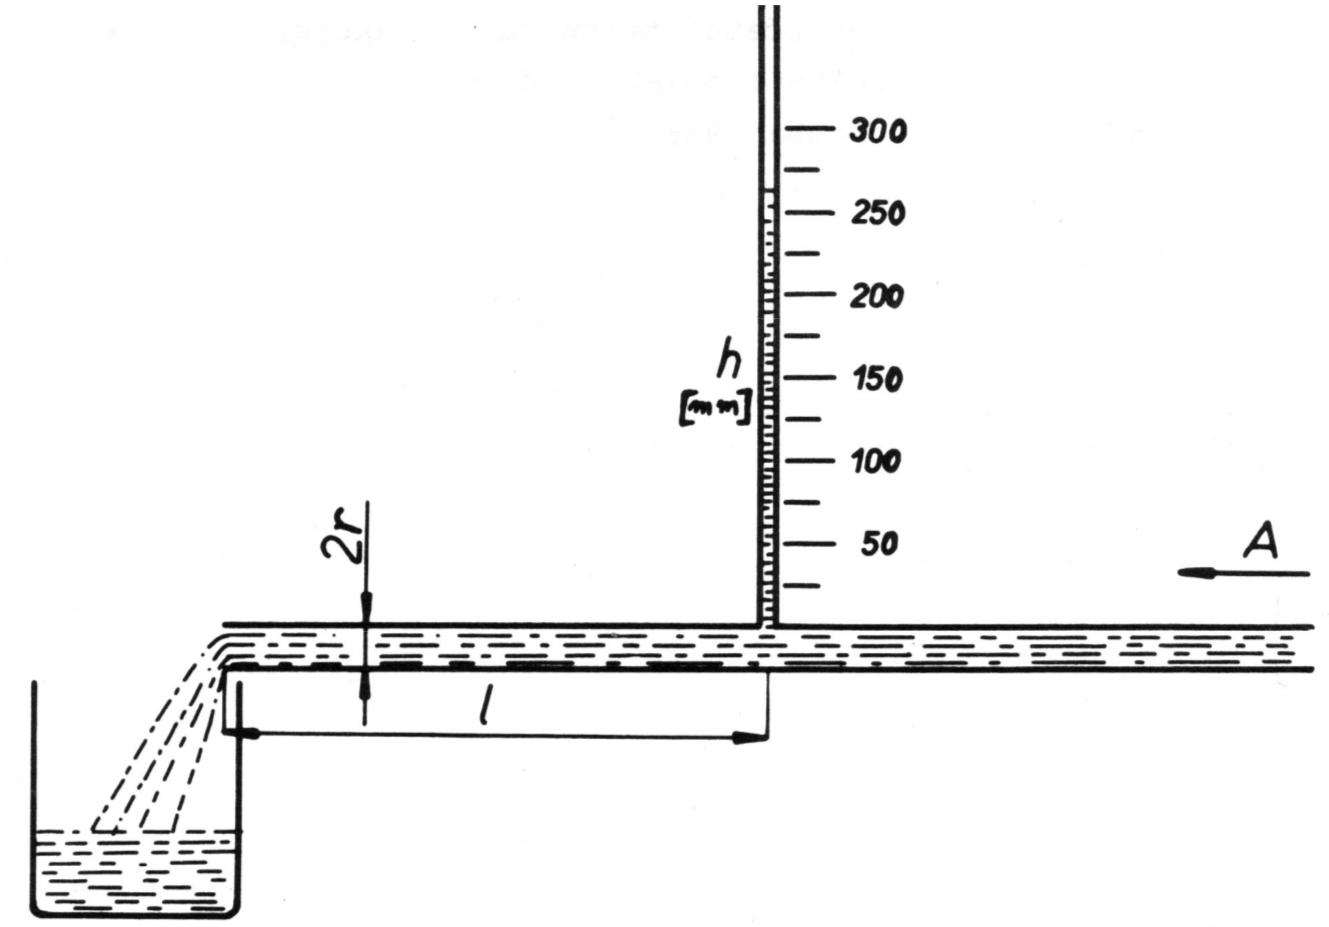
\includegraphics[width=\textwidth-2cm]{graficos/zfp}
\caption{Nákres použité aparatury (převzato z \cite{ZFP})}
\label{obr:zfp-nakres}
\end{figure}

Měříme závislost objemového průtoku $Q_v$ na úbytku statického tlaku $p$\footnote{Úbytek statického tlaku značíme $p$, zatímco $\sigma p$ značíme jeho standardní odchylku.} na délce $l$ ($Q_v=Q_v(p)$). Při určitém tlaku změříme objem vyteklé vody $V$ za dobu $t$, z toho vypočteme objemový průtok a jeho standardní odchylku podle

\begin{equation} \label{eq:Qv}
Q_v=\frac{V}{t}
\end{equation}


\begin{equation} \label{eq:chybaQv}
\sigma Q_v=Q_v \cdot \sqrt{      \left(\frac{\sigma V}{V} \right)^2+        \left(\frac{\sigma t}{t}\right)^2}
\end{equation}


Úbytek statického tlaku a jeho odchylku spočítáme z výšky vodního sloupce $h$ v manometrické trubici podle\cite{ZFP}

\begin{equation} \label{eq:tlak-na-h}
p=h\cdot \rho \cdot g
\end{equation}


\begin{equation} \label{eq:chybatlak}
\sigma p = p \cdot \sqrt{      \left(\frac{\sigma h}{h} \right)^2+        \left(\frac{\sigma \rho}{\rho}\right)^2   +   \left(\frac{\sigma g}{g}\right)^2}~,
\end{equation}
kde $\rho$ je hustota vody a $g$ je tíhové zrychlení.


Při laminárním proudění teoreticky objemový průtok závisí lineárně na úbytku tlaku, tento vztah je dán  \mbox{Poisseuillovou} rovnicí\cite{ZFP}

\begin{equation} \label{eq:poiss}
Q_v=\frac{\pi r^4}{8 \eta l} p~,
\end{equation}
kde $\eta$ je dynamická viskozita vody.

Nafitujeme tuto závislost v oblasti laminárního proudění pro každou trubici funkcí

\begin{equation} \label{eq:fit}
Q_v = a\cdot p + b
\end{equation}

Porovnáním s \eqref{eq:poiss} dostáváme

\begin{equation} \label{eq:polomer_z_a}
r=\sqrt[ 4]{\frac{8 a \eta l}{\pi}}
\end{equation}

\begin{equation}
\sigma r = \frac{1}{16} \cdot r \cdot \sqrt{      \left(\frac{\sigma a}{a} \right)^2+        \left(\frac{\sigma \eta}{\eta}\right)^2   +   \left(\frac{\sigma l}{l}\right)^2}
\end{equation}

Parametr $b$ zavádíme kvůli systematické chybě způsobené kapilárními jevy v manometrické trubici. Výška sloupce vody v \eqref{eq:tlak-na-h} neodpovídá přesně úbytku tlaku. V jedné z trubic dosahovala výška sloupce při nulovém průtoku až 1~cm.



K rozlišení laminárního a turbulentního proudění se používá Reynoldsovo číslo definované vztahem\cite{ZFP}

\begin{equation} \label{eq:reynoldsdef}
Re=\frac{r \rho v_s}{\eta}~,
\end{equation}
kde $v_s$ je střední rychlost proudění v průřezu trubice. Zřejmě platí $Q_v=\pi r^2 v_s$. Po dosazení za $v_s$ do \eqref{eq:reynoldsdef} dostáváme Reynoldsovo číslo a jeho chybu\footnote{za $r$ dosazujeme opravený poloměr z \eqref{eq:polomer_z_a}}

\begin{equation} \label{eq:reynoldsvypocet}
Re=\frac{Q_v \cdot \rho}{r \cdot \pi \cdot \eta}
\end{equation}

\begin{equation} \label{eq:reynoldschyba}
\sigma Re=Re \cdot \sqrt{      \left(\frac{\sigma Q_v}{Q_v} \right)^2+        \left(\frac{\sigma \rho}{\rho}\right)^2+        \left(\frac{\sigma r}{r}\right)^2+        \left(\frac{\sigma \eta}{\eta}\right)^2}
\end{equation}


Pokud je hodnota Reynoldsova čísla nižší než kritická hodnota (přibližně 2000 \cite{ZFP}), jedná se o laminární proudění. V rozmezí přibližně 1000--2000 \cite{ZFP} je proudění nestabilní, to se projeví vysokým rozptylem naměřených hodnot $h$ v této oblasti. Pro hodnoty vyšší než 2000 je již proudění trvale turbulentní.

Zavedeme součinitel odporu trubice $k$ a definujeme ho vztahem\cite{ZFP}

\begin{equation} \label{eq:kdef}
p=k \cdot \frac{l}{r} \cdot \frac{1}{2} \rho v_s^2
\end{equation}

Po úpravě a dosazení za $v_s$ dostáváme

\begin{equation}\label{eq:kvypocet}
k= 2\pi^2 \cdot \frac{p \cdot r^5}{l \cdot \rho \cdot Q_v^2}
\end{equation}

\begin{equation}\label{eq:kchyba}
\sigma k = k \cdot \sqrt{      \left(\frac{\sigma p}{p} \right)^2+        \left(5\frac{\sigma r}{r}\right)^2+        \left(\frac{\sigma l}{l}\right)^2+        \left(\frac{\sigma \rho}{\rho}\right)^2  +      \left(2\frac{\sigma Q_v}{Q_v}\right)^2}
\end{equation}

Porovnáním \eqref{eq:poiss}, \eqref{eq:kdef} a \eqref{eq:reynoldsdef} dostaneme pro laminární proudění

\begin{equation}\label{eq:klaminarni}
k=\frac{16}{Re}
\end{equation}

Pro turbulentní proudění se uvádí experimentálně zjistěná závislost\cite{ZFP}

\begin{equation}\label{eq:kturbulentni}
k \approx \frac{0,133}{\sqrt[4]{Re}}
\end{equation}










\section*{Podmínky a měřící přístroje}
Teplotu vody jsme změřili rtuťovým teploměrem. Vzhledem k možnému chladnutí vody během průběhu experimentu odhadujeme standardní odchylku na $1 ~\degree C$. Teplota vody byla tedy $(27 \pm 1)~ \degree C$.

Dynamická viskozita vody je při této teplotě $\eta = (0,85 ~ \pm ~0,05)~ mPa . s$ \cite{viskozita}.

Hustota vody je při této teplotě $\rho = (996~\pm~5) \cdot kg.m^{-3}$ \cite{viskozita}.

Tíhové zrychlení v Praze zaokrouhlíme na $g=(9,81 \pm 0.01) \cdot \text{m.s \textsuperscript{-2}}$ \cite{tihovyzrychleni}.

Výšku sloupce vody v manometrické trubici jsme měřili pravítkem s nejmenším dílkem $1 ~\text{mm}$. Standardní odchylku výšky sloupce odhadujeme v případě, kdy hladina nekolísá, na $\sigma h = 1~\text{mm}$ a v případě, kdy hladina kolísá, uvažujeme odchylku jako maximální změnu během daného měření.

Délku $l$ (viz obr. \ref{obr:zfp-nakres}) jsme měřili metrem s nejmenším dílkem 1~mm. Kvůli šířce manometrické trubice však odhadujeme standardní odchylku $\sigma l = 2~\text{mm}$.

Průměr trubic $r$ jsme měřili plastovým posuvným měřítkem, poloměr jsme určili jako polovinu průměru. Za standardní odchylku poloměru považujeme $\sigma r =$~0,1~mm.

Objem vytečené vody jsme měřili odměrnými válci s nejmenšími dílky 0,2~ml, 0,5~ml, 1~ml a 2~ml. Za standardní odchylku považujeme vždy nejmenší dílek.

Dobu výtoku jsme měřili stopkami s poslední zobrazenou číslicí odpovídající 0,1~s. Měření jsme prováděli tím způsobem, že při určitém čase na stopkách jsme se snažili odejmout odměrný válec od ústí trubice. Tento postup s sebou nese zřejmou nepřesnost, proto považuji standardní odchylku doby výtoku $\sigma t = \text{0,5~s}$. Tato odchylka je stejná pro všechny měření času.